\chapter{Boltzmann Machines}
This chapter gives an introduction to Boltzmann machines and their applications to the classical 
simulation of quantum computing.

An overview of the architecture and mathematical properties of Boltzmann machines are given in 
the first section. The restricted Boltzmann machine is motivated as a special kind of 
Boltzmann machine with helpful mathematical properties in the second part of this 
chapter. In the last section, a constructive approach is given on how restricted Boltzmann machines 
can be applied to the classical simulation of quantum computing.

The introduction to Boltzmann machines and restricted Boltzmann machines is based on \cite{montufar2018restricted} and 
\cite{fischer2012introduction} which are also recommended as a more throughout introduction into the topic. The 
reader who is already familiar with the concept of Boltzmann machines can safely skip
to section~\ref{sec:applicationToQuantumComputing} which is based on the work of J\'{o}nsson, Bauer and Carleo \cite{jnsson2018neuralnetwork}.

\section{Overview}
The concept of the Boltzmann machine (BM) has first been proposed in the 1980s as a
model for parallel distributed computing \cite{hinton1983analyzing}. BMs are physically inspired by the Ising Spin model 
and can be interpreted as energy based recurrent neural networks representing probability distributions
over vectors $\bm{d} \in \{0,1\}^n$ \cite{ackley1985learning}.

A Boltzmann machine is a network of stochastic units (or neurons) $X=V \cup H$ which are segmented into
\textit{visible} neurons $V=\{v_1, \dots, v_n\}$ and \textit{hidden} neurons $H=\{h_1, \dots, h_m\}$.
The joint state of the visible neurons $\bm{v} = (v_1\dots v_n) \in \{0,1\}^n$ represents data points $\bm{d}_i \in \{0,1\}^n$.
The hidden neurons increase the expressiveness of the Boltzmann machine by acting as non-linear feature 
detectors to model dependencies between the visible neurons \cite{hinton2010boltzmann}. The neurons are 
connected to each other by weighted links $W_{ij}$ and posses a bias $a_i$ or $b_i$ respectively. In the
general case, Boltzmann machines are allowed to be fully connected. A graphical 
representation of a fully connected Boltzmann machine is shown in figure~\ref{fig:boltzmannMachine}.

\begin{figure}[h]
    \label{fig:boltzmannMachine}
    \centering
    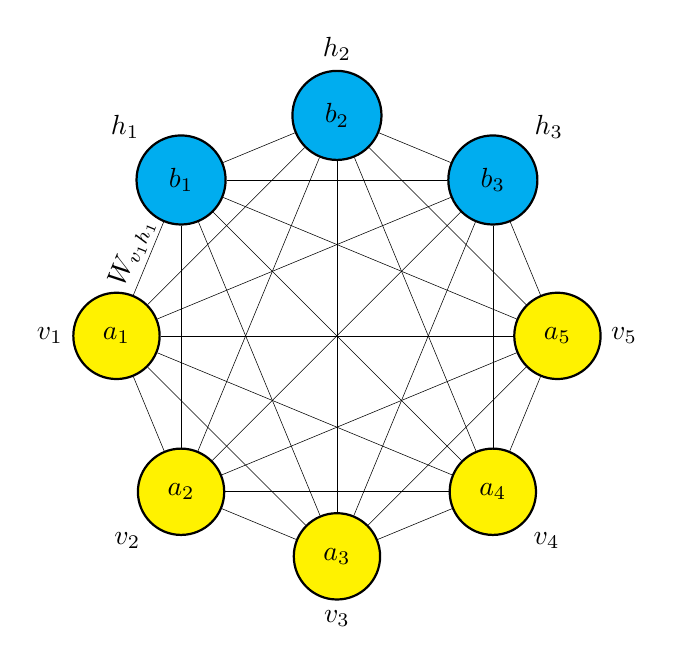
\begin{tikzpicture}[transform shape,line width=0.2pt]
        \foreach \x in {1,...,8}{%
            \pgfmathparse{(\x-1)*45+floor(\x/9)*22.5}
            \node[label={\pgfmathresult:\ifnum\x=1 $v_5$\else\ifnum\x=2 $h_3$\else\ifnum\x=3 $h_2$\else\ifnum\x=4 $h_1$\else\ifnum\x=5 $v_1$\else\ifnum\x=6 $v_2$\else\ifnum\x=7 $v_3$\else\ifnum\x=8 $v_4$\fi\fi\fi\fi\fi\fi\fi\fi},draw,circle,inner sep=0.25cm,fill={\ifnum\x=1 yellow\else\ifnum\x<5 cyan\else yellow\fi\fi}] (N-\x) at (\pgfmathresult:2.8cm) [thick] {\ifnum\x=1 $a_5$\else\ifnum\x=2 $b_3$\else\ifnum\x=3 $b_2$\else\ifnum\x=4 $b_1$\else\ifnum\x=5 $a_1$\else\ifnum\x=6 $a_2$\else\ifnum\x=7 $a_3$\else\ifnum\x=8 $a_4$\fi\fi\fi\fi\fi\fi\fi\fi};
        }
        \foreach \x [count=\xi from 1] in {2,...,8}{%
            \foreach \y in {\x,...,8}{%
                \ifnum\y=5 \else\ifnum\xi=5 \else \path (N-\xi) edge[-] (N-\y)\fi\fi;
            }
        }
        \draw (N-5) -- (N-1) node [] (E-1) {};
        \draw (N-5) -- (N-2) node [] (E-2) {};
        \draw (N-5) -- (N-3) node [] (E-3) {};
        \draw (N-5) -- (N-4) node [midway,above=-0.06cm,sloped] (E-4) {$W_{v_{1}h_{1}}$};
        \draw (N-5) -- (N-6) node [] (E-5) {}; 
        \draw (N-5) -- (N-7) node [] (E-6) {};
        \draw (N-5) -- (N-8) node [] (E-7) {};
    \end{tikzpicture}
    \caption{Graphical representation of a fully connected Boltzmann machine with 5 visible neurons (yellow) $v_1$ to $v_5$
    and 3 hidden neurons (blue) $h_1$ to $h_3$. Each neuron posses a bias
    $a_1$ to $a_5$ and $b_1$ to $b_3$ respectively. The connection weight between two neurons $i$ and $j$
    is given by $W_{ij}$.}
\end{figure}

Each configuration $\bm{c}=(v_1,\dots,v_n,h_1,\dots,h_m)$ of neuron states
of the Boltzmann machine is associated with an energy $E(\bm{c})$ value
which is defined by its weights and biases $\mathcal{W} = \{a_i, b_i, W_{ij}\}$:

\begin{equation}
  E(\bm{c};\mathcal{W}) = - \sum_{v_i \in V} a_{i}v_{i} - \sum_{h_i \in H} b_{i}h_{i} - \sum_{x_i,x_j \in X} W_{x_i,x_j}x_{i}x_{j}
\end{equation}

When sampling configurations from the Boltzmann machine (discussed in more detail in section~\ref{sec:gibbsSampling}) the 
Boltzmann machines prefers low energy states over states with a high energy. The stationary probability
of a configuration $\bm{c}$ with energy $E(\bm{c};\mathcal{W})$ is given by the so called Gibbs-Boltzmann distribution \cite{gibbs_2010}:

\begin{equation}
   p(\bm{c};\mathcal{W}) = \frac{\mathrm{e}^{-E(\bm{c};\mathcal{W})}}{Z(\mathcal{W})}
\end{equation}

where $Z(\mathcal{W})$ is the normalizing partition function 

\begin{equation}
   Z(\mathcal{W}) = \sum_{\bm{c}\prime\in C} \mathrm{e}^{-E(\bm{c}\prime;\mathcal{W})}
\end{equation}

In a training phase the parameters of the Boltzmann machine can be adapted in such a way that 
the marginal probability distribution of the visible neurons which traces out the hidden unit 
states by summing over all possible configurations of them:

\begin{equation}
   p(\bm{v};\mathcal{W}) = \sum_{\bm{h}_k \in \{0,1\}^m} p(\bm{v},\bm{h}_k;\mathcal{W})
\end{equation}

resembles the probablity distribution of data points $d_i$ in a training set $D=\{d_1,\dots,d_l\}$.
For a fully connected Boltzmann machine this representation consists of an exponential number of 
summands and thus cannot be calculated efficiently. So called Restricted Boltzmann machines
(RBM) have a specific architecture with a restricted connectivity which makes the representation 
of the marginal probability compact as will be shown in the next section.

\section{Restricted Boltzmann machines}
The so called Restricted Boltzmann machine (RBM) is an important type of Boltzmann machine with 
a specific architecture and properties \cite{smolensky1986information}. Since their invention RBMs have been applied to variety 
of machine learning tasks. They also played a 
key role in the development of deep learning architectures as building blocks of so called 
Deep Belief networks \cite{bengio2009learning, hinton2006fast}.
RBMs are also the kind of Boltzmann machines which are being used in this study for the simulation 
of quantum circuits.

\subsection{Properties}

In the restricted case the neurons of the Boltzmann machine are seperated into two layers of visible and hidden neurons which form a bipartite graph. There 
are only connections allowed between the neurons from the two different layers and no intra-layer connections. The structure of an 
RBM is shown in figure~\ref{fig:rbm}. 

\begin{figure}[h]
    \label{fig:rbm}
    \centering
    \begin{tikzpicture}[transform shape,line width=0.2pt]
    
        \node (v1)[neuron, fill=yellow] at (0, 0) {$a_1$};
        \node (v2)[neuron, fill=yellow] at (2, 0) {$a_2$};
        \node (v3)[neuron, fill=yellow] at (4, 0) {$a_3$};
        \node (v4)[neuron, fill=yellow] at (6, 0) {$a_4$};
        \node[below=0.1cm of v1] (bv1) {$v_1$};
        \node[below=0.1cm of v2] (bv2) {$v_2$};
        \node[below=0.1cm of v3] (bv3) {$v_3$};
        \node[below=0.1cm of v4] (bv4) {$v_4$};
    
        \node (h1)[neuron, fill=cyan] at (1, 2) {$b_1$};
        \node (h2)[neuron, fill=cyan] at (3, 2) {$b_2$};
        \node (h3)[neuron, fill=cyan] at (5, 2) {$b_3$};
        \node[above=0.1cm of h1] (bh1) {$h_1$};
        \node[above=0.1cm of h2] (bh2) {$h_2$};
        \node[above=0.1cm of h3] (bh3) {$h_3$};
    
        \draw (v1) -- (h1) node [midway,above=-0.06cm,sloped] {$W_{v_1h_1}$};
        \draw (v1) -- (h2) node [midway,above=-0.06cm,sloped] {};
        \draw (v1) -- (h3) node [midway,above=-0.06cm,sloped] {};
    
        \draw (v2) -- (h1) node [midway,above=-0.06cm,sloped] {};
        \draw (v2) -- (h2) node [midway,above=-0.06cm,sloped] {};
        \draw (v2) -- (h3) node [midway,above=-0.06cm,sloped] {};
    
        \draw (v3) -- (h1) node [midway,above=-0.06cm,sloped] {};
        \draw (v3) -- (h2) node [midway,above=-0.06cm,sloped] {};
        \draw (v3) -- (h3) node [midway,above=-0.06cm,sloped] {};
    
        \draw (v4) -- (h1) node [midway,above=-0.06cm,sloped] {};
        \draw (v4) -- (h2) node [midway,above=-0.06cm,sloped] {};
        \draw (v4) -- (h3) node [midway,above=-0.06cm,sloped] {};
    \end{tikzpicture}
    \caption{Graphical representation of a RBM with 5 visible neurons and 3 hidden ones. 
    There are only connections between the two layers and no connection within one of the 
    layers.}
\end{figure}

The marginal probability of the visible neuron states in an RBM has a closed form:

\begin{align}
   p(\bm{v};\mathcal{W}) &= \sum_{\bm{h}_k \in \{0,1\}^m} p(\bm{v},\bm{h}_k;\mathcal{W})\\
   &= \frac{1}{Z(\mathcal{W})}\sum_{\bm{h}_k \in \{0,1\}^m} \mathrm{e}^{-E(\bm{v}, \bm{h}_k;\mathcal{W})}\\
   &= \frac{1}{Z(\mathcal{W})}\sum_{h_1\in \{0,1\}}\dots\sum_{h_m \in \{0,1\}}\mathrm{e}^{\sum_{v_i}b_iv_i}\prod_{j=1}^m\mathrm{e}^{h_j(b_j + \sum_{i=1}^nW_{ij}v_i)}\\
   &= \frac{\mathrm{e}^{\sum_{v_i}b_iv_i}}{Z(\mathcal{W})}\sum_{h_1 \in \{0,1\}}\mathrm{e}^{h_1(b_1 + \sum_{i=1}^nW_{i1}v_i)}\dots\sum_{h_m \in \{0,1\}}\mathrm{e}^{h_m(b_m + \sum_{i=1}^nW_{im}v_i)}\\
   &= \frac{\mathrm{e}^{\sum_{v_i}b_iv_i}}{Z(\mathcal{W})}\prod_{i=1}^m\sum_{h_i \in \{0,1\}}\mathrm{e}^{h_i(b_i + \sum_{i=1}^nW_{ij}v_i)}\\
   &= \frac{\mathrm{e}^{\sum_{v_i}b_iv_i}}{Z(\mathcal{W})}\prod_{i=1}^m(1+\mathrm{e}^{b_i + \sum_{i=1}^nW_{ij}v_i})
\end{align}

This quantity consists of only a polynomial number of terms in the number of hidden units of the RBM and 
thus can be calculated efficiently.

Before it will be shown how those probabilities can be used sample from the configurations of the neuron states
of the Boltzmann machine in section~\ref{sec:gibbsSampling}, a short excursion on the Representational power 
of BMs and RBMs is made in the next section.

\subsection{Representational Power}
\section{Supervised Learning}
\subsection{Gibbs Sampling}
\label{sec:gibbsSampling}
Boltzmann machines are generative models that represent probability distributions over its configurations.
The probability for a configuration $\bm{c}$ has been given in equation X and X for fully connected and 
restricted Boltzmann machines respectively. The process on how to draw such configurations of joint 
probabilities of the BMs state is called \textit{Gibbs Sampling}.

Gibbs sampling belongs to the class of so called \textit{Metropolis-Hastings} algorithms \cite{}.
It is a simple algorithm to produce samples from the joint probability distribution of multiple random
variables as in the case of neuron states of a Boltzmann machine. The joint configuration of neuron states
is considered as a \textit{Markov Chain}.

A Markov chain is a discrete stochastic process of random variables $X=\{x_1,\dots,x_n\}$ which take values 
in a (in the following considerations finite) set $\Omega$ and for which $\forall k \geqq 0$ and 
$\forall j,i,i_0,\dots,i_{k-1} \in \Omega$ the \textit{Markov property} holds:

\begin{align}
    p_{ij}^{(k)} &:=P(X^{(k+1)}=j \mid X^{(k)} = i, X^{(k-1)} = i_{k-1}, \dots, X^{(0)} = i_0) \\
                 & =P(X^{(k+1)}=j \mid X^{(k)} = i) 
\end{align}

meaning that the next state of the system only depends on the current state and not on the history of 
the system.

A distribution $\pi$ for which it holds that $\pi^T=\pi^TP$ is called \textit{stationary distribution}.
If the Markov chain for any time $k$ reaches the stationary distribution $\mu^{(k)}= \pi$ all subsequent
states will be distributed accordingly, that is, $\mu^{(k+n)}=\pi$ for all $n \in \mathbb{N}$.
A sufficient (but not necessary) condition for a distribution $\pi$ to be stationary w.r.t. a Markov 
chain described by the transition probabilities $p_{ij},i,j \in \Omega$ is that $\forall i,j \in \Omega$ 
it holds:

\begin{equation}
    \pi(i)p_{ij}= \pi(j)p_{ij}
\end{equation}

This is called the \textit{detailed balance condition}.

Especially relevant are Markov chains for which it is known that there exists an unique stationary distribution.
For finite $\Omega$ this is the case if the Markov chain is \textit{irreducible}. A Markov chain is 
irreducible if one can get from any state in $\Omega$ to any other in a finite number of transitions or 
more formally $\forall i, j \in \Omega \exists k > 0$ with $P(X^{(k)}=j \mid X^{(0)=i}) >0$.

A chain is called \textit{aperiodic} if for all $i \in \Omega$ the greatest common divisor of $\{k \mid P(X^{(k)} = i \mid
X^{(0)} = i) > 0 \land k \in \mathbb{N}_0\}$ is 1. One can show that an irreducible and aperiodic Markov 
chain on a finite state space is guarantied to converge to its stationary distribution (see, e.g. \cite{}).
That is, for an arbitrary starting distribution $\mu$ it holds

\begin{equation}
    lim \dots = 0
\end{equation}

where $d_V$ is the \textit{distance of variation}. For two distributions $\alpha$ and $\beta$ on a 
finite state space $\Omega$, the distance of variation is defined as 

\begin{equation}
d_V= \dots
\end{equation}

.

In the case of Boltzmann machines, the transition probability $\pi_{ij}$ from one configuration $c_i$ to another
configuration $c_j$ is given by the ratio of their respective state probabilities:

\begin{equation}
    \pi_{ij} = \dots
\end{equation}

The Markov chain defined by these probabilities fullfills the detailed balance condition and thus 
has a stationary distribution. show irreducible and aperiodic implying stationary.

During the Gibbs sampling at each timestep $t$ the state of a randomly chosen unit of the BM is flipped.
Afterwards, the transition probability of the old an new configuration is computed as in ??. The new 
configuration will be kept with that probability and be reverted to stay in the old configuration with 
probability 1-... . After enough time steps t, the configuration of the Boltzmann machine converges to 
its stationary distribution. 

Running the Gibbs sampling multiple times for a fixed amount of timesteps $T$, samples from it can be 
drawn.

\subsection{Gradient Descent}
\section{Application to Quantum Computing}
\label{sec:applicationToQuantumComputing}
Boltzmann machine have been shown to be a good model for quantum physics. Carleo used RBMs to predict the wave functions 
of many body quantum states in X. Xiao could show that while General Boltzmann machines can represent the wave functions of 
many body systems directly, sampling becomes the P Sharp problem mentioned above. Restricted Boltzmann machines in contrast 
are not able to represent the exact states but can approach them reasonable well with a worst case inefficient representation 
but with an efficient sampling process. Carleo et al later used restriced Boltzmann machines for the classical simulation of 
quantum computing. This is the framework this study builds on top and will be explained in greater detail in this section.

With the concept of the RBM at hand the question remains how it can be used to represent the states of indivual qubits. The
link is that as the wavefunction assigns an energy value to each state so does the Boltzmann machine assign an energy value 
to each state of visible units by formular X.

The state that is represented by the Boltzmann machine is therefore given by the superposition of possible state and their 
corresponding energy values:

FORMULAR

For the representation of quantum states the weights and biases of the RBM will be complex valued.

All gates which are diagonal in the computational basis can be applied by following rules to update the parameters of the RBM
in order to satisfy the equations for the RBM. Non-diagonal gates can be approximated by training the Boltzmann machine to 
learn the state after the gate has been applied to the currently represented state of the RBM.

\subsection{Diagonal gates}
\subsubsection{Single-Qubit Z rotations}
The action of the single Z rotation of angle $\theta$ is given by the $2\times2$ unitary matrix

\begin{equation}
    \begin{pmatrix}
        1 & 0 \\
        0 & \mathrm{e}^{i\theta}
    \end{pmatrix}
\end{equation}

Its action on qubit $l$ yields 
$\langle \mathfrak{B} \mid R_{l}^{z}(\theta) \mid \Psi_{W}  \rangle = 
\mathrm{e}^{i\theta B_{l}} \Psi_{W}(\mathfrak{B})
$
. Considering a RBM machine with weights $W\prime = \{\alpha,\beta,W\}$, the action of the $R^{Z}{\theta}$
gate is exactly reproduced if we satisfy $\mathrm{e}^{B_{l}a_{l}}\mathrm{e}^{i\theta B_{l}} = \mathrm{e}^{B_{l}a\prime_{l}}$,
which has the simple solution:

\begin{equation}
    a\prime_{j} = a_{j} + \delta_{jl}i\theta
\end{equation}

The action of this gate then simply modifies the local visible bias of the RBM.

\subsubsection{Controlled Z rotations}
The action of a controlled Z rotations acting on two given qubits $l$ and $m$ is determined by
the $4\times4$ unitary matrix:

\begin{equation}
    \begin{pmatrix}
        1 & 0 & 0 & 0 \\
        0 & 1 & 0 & 0 \\
        0 & 0 & 1 & 0 \\
        0 & 0 & 0 & \mathrm{e}^{i\theta}
    \end{pmatrix}
\end{equation}

where $\theta$ is a given rotation angle. This gate is diagonal and we can compactly write it as an 
effective two-body interaction:

\begin{equation}
    \langle \mathfrak{B} \mid CZ(\theta) \mid \Psi_{W}  \rangle = 
    \mathrm{e}^{i\theta B_{l}B_{m}}\Psi_{W}(Z_{1} \dots Z_{N})
\end{equation}

Since in the RBM architecture there is no direct interaction between visible spins, this CZ interaction
can be mediated through the insertion of a dedicated extra hidden unit $h_{c}$ which is coupled only 
to the qubits $l$ and $m$: 

\begin{equation}
    \langle \mathfrak{B} \mid CZ(\theta) \mid \Psi_{W}  \rangle = 
    \mathrm{e}^{\Delta a_{l} B_{l} + \Delta a_{m} Z_{m}} \sum_{h_{c}}\mathrm{e}^{W_{lc} B_{l} h_{c} + W_{mc} B_{m} h_{c}}
\end{equation}

\begin{equation}
    = \mathrm{e}^{\Delta a_{l} B_{l} + \Delta a_{m} B_{m}} \times (1 + \mathrm{e}^{W_{lc} B_{l} + W_{mc}} B_{m}) \Psi_{W}(\mathfrak{B})
\end{equation}
, where the new weights $W_{lc}$ and $W_{mc}$ and visible units biases $a_{l}\prime= a_{l} + \Delta a_{l}$,
$a_{m}\prime= a_{m} + \Delta a_{m}$ are determined by the equation:

\begin{equation}
   \mathrm{e}^{\Delta a_{l} B_{l} + \Delta a_{m} B_{m}}(1 + \mathrm{e}^{W_{lc} B_{l} + W_{mc} B_{m}}) = C \times \mathrm{e}^{i \theta B_{l} B_{m}} 
\end{equation}
, for all the four possible values of the qubits values $B_{l}, B_{m} = \{0,1\}$ and where $C$ is an arbitrary (finite)
normalization. A possible solution for this system is:

\begin{equation}
   W_{lc} = -2\mathrm{A}(\theta) 
\end{equation}

\begin{equation}
   W_{mc} = 2\mathrm{A}(\theta) 
\end{equation}

\begin{equation}
   \Delta a_{l} = i \frac{\theta}{2} + \mathrm{A}(\theta)
\end{equation}

\begin{equation}
   \Delta a_{m} = i \frac{\theta}{2} - \mathrm{A}(\theta)
\end{equation}

where $\mathrm{A}(\theta) = arccosh(\mathrm{e}^{-i \frac{\theta}{2}})$

\subsubsection{Pauli X gate}
We then consider a $X$ gate acting on some given qubit $l$. In this case the gate just flips the qubit
and the RBM amplitudes are:

$
    \langle \mathfrak{B} \mid X_{l} \mid \Psi_{W}  \rangle = 
    \langle B_{1} \dots B_{l}\bar \dots B_{N} \mid \Psi_{W}
$
,

therefore since $B_{l}\bar = (1-B_{l})$, we must satisfy 

\begin{equation}
    (1-B_{l})W_{lk} + b_{k} = B_{l} W_{lk}\prime + b_{k}\prime
\end{equation},

\begin{equation}
   (1-B_{l}) a_{l} = B_{l} a_{l}\prime + C 
\end{equation},

for all the (two) possible values of $B_{l} = \{0,1\}$. The solution is simply:

\begin{equation}
   W_{lk}\prime = -W_{lk}
\end{equation}

\begin{equation}
   b_{k}\prime = b_{k} + W_{lk}
\end{equation}

\begin{equation}
   a_{l}\prime = -a_{l}
\end{equation}

\begin{equation}
   C = a_{l}
\end{equation}

whereas all the $a_{j}$ and the other weights $W_{jk}$ with $j \neq i$ are unchanged.

\subsubsection{Pauli Y gate}
A similar solution is found also for the $Y$ gate, with the noticeable addition of extra phases
with respect to the $X$ gate:

\begin{equation}
   W_{lk}\prime = -W_{lk}
\end{equation}

\begin{equation}
   b_{k}\prime = b_{k} + W_{lk}
\end{equation}

\begin{equation}
   a_{l}\prime = -a_{l} + i \pi
\end{equation}

\begin{equation}
   C = a_{l} + \frac{i \pi}{2}
\end{equation}

whereas all the $a_{j}$ and other weights $W_{jk}$ with $j \neq l$ are unchanged.

\subsubsection{Pauli Z gate}
For a $Z$ gate acting on qubit $l$ we have:

\begin{equation}
    \langle \mathfrak{B} \mid Z_{l} \mid \Psi_{W}  \rangle = 
    (-1)^{B_{l}} \langle \mathfrak{B} \mid \Psi_{W} \rangle
\end{equation}

therefore we must satisfy $\mathrm{e}^{B_{l}a_{l}}(-1)^{B_{l}} = \mathrm{e}^{B_{l}a_{l}\prime}$, which
has the simple solution:

\begin{equation}
    a_{l}\prime = a_{l} + i \pi
\end{equation},

whereas all the other weights and biases are unchanged.

\subsection{Non-diagonal gates}
While diagonal gates can be applied as shown for the gates above by solving the corresponding sysem of linear equations, 
there are no such rules for non-diagonal gates (why not?). Instead, the effect of non-diagonal gates on a qubit l have to be 
learned with the following framework.

Any non diagonal unitary of the form 

\begin{equation}
    \begin{pmatrix}
        a & b \\
        c & d
    \end{pmatrix}
\end{equation}

has the effect that when applied to qubit l currently in state 0: ... and ... when qubit l is currently in state 1. This means 
with the current RBM at hand we can sample from the state after the gate has been applied by sampling from the current state 
and adapting the wave function accordingly. This can be done efficiently as it is a simple addition of two wave function values 
which in turn can be calculated efficiently as well. This approach allows us to generate a training set with samples of the 
after gate state and the corresponding target wave function values. This training set can be used to minimize the overlap of
the current and the target state:

For numerical reasons, it is a common trick to not minimize the bare overlap but the log of the overlap:

FORMULAR

which attains a minimum at .... The derivate of the log likelihood with respect to paramter k of the Boltzmann machine then 
reads as:

FORMULAR

which can be calculated efficently. Using a gradient descent the parameters can be updated in such a way to minimize the log
overlap and approach the desired state.

In their work, Carleo et al tested the framework on a fast fourier transform by applying ... . They could find a per gate 
error of 10 to the minus three, which is similar to the one currently archivable by physical quantum computers \cite{}.